%% 
%% Copyright 2007, 2008, 2009 Elsevier Ltd
%% 
%% This file is part of the 'Elsarticle Bundle'.
%% ---------------------------------------------
%% 
%% It may be distributed under the conditions of the LaTeX Project Public
%% License, either version 1.2 of this license or (at your option) any
%% later version.  The latest version of this license is in
%%    http://www.latex-project.org/lppl.txt
%% and version 1.2 or later is part of all distributions of LaTeX
%% version 1999/12/01 or later.
%% 
%% The list of all files belonging to the 'Elsarticle Bundle' is
%% given in the file `manifest.txt'.
%% 
%% Template article for Elsevier's document class `elsarticle'
%% with harvard style bibliographic references
%% SP 2008/03/01

%\documentclass[preprint,12pt,authoryear]{elsarticle}  %default in the template
%\documentclass[preprint,10pt,authoryear]{elsarticle}

%% Use the option review to obtain double line spacing
%% \documentclass[authoryear,preprint,review,12pt]{elsarticle}

%% Use the options 1p,twocolumn; 3p; 3p,twocolumn; 5p; or 5p,twocolumn
%% for a journal layout:
%% \documentclass[final,1p,times,authoryear]{elsarticle}
%% \documentclass[final,1p,times,twocolumn,authoryear]{elsarticle}
 \documentclass[final,3p,times,authoryear]{elsarticle}
%% \documentclass[final,3p,times,twocolumn,authoryear]{elsarticle}
%% \documentclass[final,5p,times,authoryear]{elsarticle}
%% \documentclass[final,5p,times,twocolumn,authoryear]{elsarticle}

%% For including figures, graphicx.sty has been loaded in
%% elsarticle.cls. If you prefer to use the old commands
%% please give \usepackage{epsfig}

%% The amssymb package provides various useful mathematical symbols
\usepackage{amssymb}
%% The amsthm package provides extended theorem environments
\usepackage{amsthm}
\usepackage{amsmath}
\usepackage{color, colortbl}
\usepackage{amsmath}
\usepackage{siunitx}
%\usepackage{todonotes}
\usepackage{tabularx}
\usepackage[]{algorithm2e}
\usepackage{soul}
%\usepackage[colorinlistoftodos]{todonotes}

\usepackage{glossaries}
\usepackage{subfig}

\usepackage{xargs}
\usepackage[pdftex,dvipsnames]{xcolor}
\usepackage[colorinlistoftodos,prependcaption,textsize=tiny]{todonotes}
\newcommandx{\unsure}[2][1=]{\todo[linecolor=red,backgroundcolor=red!25,bordercolor=red,#1]{#2}}
\newcommandx{\change}[2][1=]{\todo[linecolor=blue,backgroundcolor=blue!25,bordercolor=blue,#1]{#2}}
\newcommandx{\info}[2][1=]{\todo[linecolor=OliveGreen,backgroundcolor=OliveGreen!25,bordercolor=OliveGreen,#1]{#2}}
\newcommandx{\improvement}[2][1=]{\todo[linecolor=Plum,backgroundcolor=Plum!25,bordercolor=Plum,#1]{#2}}
\newcommandx{\thiswillnotshow}[2][1=]{\todo[disable,#1]{#2}}

\definecolor{light-gray}{gray}{0.9}

\usepackage{framed} % Framing content
\usepackage{multicol} % Multiple columns environment


\DeclareRobustCommand{\hlgreen}[1]{{\sethlcolor{green}\hl{#1}}}

\journal{TBD}
\makeglossaries


\begin{document}

%\runninghead{Nice et al.}

\title{Isolating the impacts of urban form and fabric from geography in assessing heat mitigation strategies }

\author[melb]{Kerry~A.~Nice\corref{cor1}}
\cortext[cor1]{Principal corresponding author}
\ead{kerry.nice@unimelb.edu.au}
%\author[melb]{et al.}
\author[arc,built,city]{Negin Nazarian}
\author[arc]{Mathew J. Lipson}
\author[arc]{Melissa A. Hart}
\author[melb]{Sachith Seneviratne}
\author[melb]{Jason Thompson}
\author[melb,eng]{Mark Stevenson}
\address[melb]{Transport, Health, and Urban Design Research Lab, Faculty of Architecture, Building, and Planning, University of Melbourne, Australia.}
\address[arc]{ARC Centre of Excellence for Climate Extremes, University of New South Wales, Sydney, NSW, Australia.}
\address[built]{School of Built Environment, University of New South Wales, Sydney, NSW, Australia.}
\address[city]{City Futures Research Centre, University of New South Wales, Sydney, NSW, Australia.}
\address[eng]{Melbourne School of Engineering; and Melbourne School of Population and Global Health, University of Melbourne, Australia.}







\begin{abstract}

As risks to public health due to heat stress in cities increase due to increased urbanisation and climate change, designing strategies for urban heat mitigation and to ensure that future development is climate sensitive is becoming more urgent. While urban heat can be influenced by the built and natural form of cities as well as urban activities and regional geographic settings, evaluating the effectiveness of strategies based on the built and natural forms are difficult to separate from the interactions of the geographic influences. To address this, we performed a comprehensive urban form analysis, covering the full range of realistic built and natural forms (buildings, roads, grass, and trees as well as building and vegetation heights) in cities combined with a combination of mitigation strategies, to determine the importance and relative influence of each on thermal performance. We find that during the daytime, higher air and UTCI temperatures are strongly driven by increased street fractions, with air temperatures increasing up to 10 and 15$^{\circ}$C as street fractions increase to 80 and 90\%. Reductions in air temperature of 5$^{\circ}$C are seen when increasing grass and tree fractions from 0 to 100\%. Similar patterns are seen with UTCI, with increasing street fractions of 80\% and 90\% driving increases of 6 and 12$^{\circ}$C. Following from this analysis, we demonstrate an application of the analysis by scaling up the results to city-wide heat maps of a number of Australian cities showing the impact of present day urban form, isolated from geography, topography, and local weather conditions. The resulting method allows mitigation strategies to be tested based on elements that are possible to be changed (the urban form) and removed from the elements that cannot be redesigned.





%Strategies for urban heat mitigation often make broad and non-specific recommendations (i.e. plant more trees) without accounting for local context. 

%\todo[inline]{Negin Nazarian: suggest detailing what "local context" may refer to.  For instance, regional geographic setting (lat/lon, distance from the coast, terrain) as well as background climate?  \\ -- thinking about this again, the local context that I listed here is in fact not correct. Please see my lengthy note below. nonetheless, need to clarify} 

%As a result, resources might be allocated to areas of lesser need over those where more urgent interventions are needed. Also, these interventions might return less than optimal results if local conditions are not considered. This project aims to assist with these interventions by providing a method to examine the urban heat profile of a city through an automated systematic approach. 

%  

%\todo[inline]{Negin Nazarian: May I suggest that we rephrase the emphasis of the paper? \\ What I suggest is that we briefly note that canopy temperature and heat stress depend on 4 categories of parameters (taken from WMO work we are doing as well as Masson et al 2020): 1) built form, 2) natural and vegetated form (including soil, water, vegetation, and phenology of all), 3) urban "function" that covers human impacts, and 4) regional geographic settings.  Of these, (1) and (2) are often the focus of mitigation measures for urban heat. \\ -- However, the interaction between these parameters, and their compounding effect on canopy T and HS, is non-linear. This complex interaction makes it hard to quantify the impact of mitigation measures in different cities with distinct urban form and functions and more importantly, distinguish this impact from regional geographical settings. \\ -- To address this shortcoming, there is a need for a comprehensive set of sensitivity analyses that cover a combination of mitigation strategies with realistic built and natural forms existing in cities. So far, such sensitivity analyses are only done to a very limited extent  (focused on limited parameters or times of the day) motivating our current work to simulate XX many scenarios covering YY many parameters for moderate and extreme summer heat. This includes the most comprehensive  set of simulations that quantifies the sensitivity of canopy T and UTCI to a combination of design parameters. Using this method, the impact of mitigation strategies can be isolated from regional geographic settings (that has been impossible for instance with mesoscale simulations). \\ --Thinking about this again, the local context that I listed here is in fact not correct. Please see my lengthy note below. nonetheless, need to clarify}


\end{abstract}

\begin{keyword}
micro-climate\sep 
urban morphology\sep
urban heat
\end{keyword}



\maketitle

\section{Introduction}

\subsection{Need for urban heat mitigation measures}

Measures of cumulative heat show significant increases in recent decades with trends of increased heatwave frequency and duration seen in almost all regions in the world \citep{Perkins-Kirkpatrick2020}. Exposure to dangerous levels of heat stress are expected to increase globally by a factor of 5-10 by 2080 \citep{Coffel2018}, driven by more frequent, severe, and long-lasting heatwaves \citep{IPCC2013a}. Heat in urban areas is the most dangerous natural hazard in Australia \citep{Coates2014}, with disproportionate risks falling on vulnerable populations such as elderly and the very young \citep{Nicholls2008}. The design of cities has enhanced these risks by replacing natural pervious land covers with hard heat absorbent surfaces, resulting in increased heat stress for those who live in cities \citep{Coutts2012,Martilli2020}. This urbanisation of land-use has altered the urban energy balance \citep{Oke1982}. Anthropogenic waste heat from buildings and transport and reduced shading through diminishing tree canopy cover result in larger amounts of net energy at street level. Meanwhile, the conversion of vegetated to impervious surfaces and the reduction of available water in cities shifts the urban energy balance away from latent heat (water evaporation) towards increased sensible heat (heat that can be felt) and increased heat storage in urban surfaces. 

Mitigation strategies that incorporate findings from urban climate research into planning of future development can ensure that new built areas are climate sensitive and better able to address the adverse effects of urban design on the thermal environment. These strategies, which rely on modifications to built form, fabric, and natural land cover in cities, require both an understanding of the processes driving excess heat, and the methods required to identify the existing areas of high risk that will benefit most from interventions. \cite{Krayenhoff2021}, in a systematic review, identified commonly used urban heat mitigation strategies, including cooling through albedo changes, vegetation cover, irrigation and water, and photovoltaic panels. Albedo changes, increasing the reflectivity of urban surfaces, can reduce road and sidewalk surface temperatures but may cause increased radiant loads for pedestrians \citep{Middel2020}. If applied at roof levels, albedo changes can provide urban heat reductions \citep{Jacobs2018Roof}. Urban vegetation provides cooling benefits through shading of urban surfaces and evapotranspiration \citep{Bowler2010,Coutts2012,Coutts2015}, as well as reducing hard impervious surfaces in favour of pervious vegetated surfaces \citep{Middel2019a}. Additional cooling can also be realised through irrigation of both vegetated \citep{Broadbent2017a,Cheung2021} and impervious surfaces \citep{Hendel2016,Solcerova2018}.


In a review of the influence of cities on local meteorology, \cite{Masson2020a} find that urban climates and heat stress in cities are influenced by four main factors, 1) the built form, 2) the natural and vegetated form (i.e. soil, water, vegetation and their phenology), 3) urban functions (heat released by human activities), and 4) regional geographic settings. As noted above, (1) and (2) are often the focus of mitigation strategies. However, the interaction of the different elements of urban form as well as the compounding effect on canopy temperatures and heat stress are often non-linear. The complexity of these interactions makes quantifying the impact of each mitigation measure difficult across different cities and their individual mixes of urban form. Additionally, each city's regional geography (including topography and distance from and orientation to an ocean) adds additional complexity in separating the impact of mitigation measures from the geography influence. 

\subsection{Metrics to assess urban heat mitigation measures}

Assessing the effectiveness of cooling strategies requires metrics to measure urban heat. These metrics need to account for different scales and carefully chosen for the intended purpose. Scales used to assess urban climates are commonly defined \citep{Oke2017} as a mesoscale (10km and greater), a micro-scale which provides an `in-street' climate (under 1km), and an overlapping local scale between the two (100m to tens of kms). Air temperatures will show the least variability in nearby locations across a neighbourhood or precinct, for example, \cite{Coutts2015} finds air temperature differences of approximately 1.5$^{\circ}$C between two adjoining identical street canyons varying only by the level of canopy cover (an open canopy vs. much more extensive tree cover). Air temperatures can be measured using simple equipment, however more extensive observations of variability across a local area requires a dense network of instruments \citep{Potgieter2021}, as well as additional information required to untangle the local weather conditions or topography from the influence of the urban form. 

Surface temperatures, on the other hand, can show wide ranges in variability across a micro-scale depending on the surface types and whether the surfaces are shaded or not. Surface temperatures of shaded surfaces will be similar to the surrounding air temperatures while nearby unshaded surfaces can be 20-30$^{\circ}$C hotter. Remotely sensed land surface temperatures (LST) can be observed using satellite or aircraft, quickly mapping wide areas, but are limited to the fly-over time. LST has often been used to identify hotspots \citep{Aniello1995} or to evaluate cooling strategies \citep{Zhu2012a,Duncan2018,Manoli2019,Ossola2021}, however the validity of these results and the ability to link LST, which is measured at the top of the urban canopy, to thermal comfort at ground level can be limited and misleading \citep{Coutts2016d}. As the shading provided by the urban canopy (both vegetation and urban structures) is a significant cooling mechanism \citep{Coutts2015,Lee2018,Krayenhoff2021}, these effects will not be captured in an above canopy assessment. Obtaining under canopy surface temperature observations of these heterogeneous environments is challenging, time consuming and limited in scale and resolution and to the observation time period \citep{Middel2019a}. To capture all the influences of urban geometry and materials on human thermal comfort, especially the influences on mean radiant temperature \citep{Kantor2011} (a temperature that accounts for the thermal stresses on a person from both solar exposure and energy/heat radiating from nearby surfaces), requires micro-scale observations and specialised equipment. Finally, human thermal comfort (HTC) indexes such as the Universal Thermal Climate Index (UTCI) \citep{Brode2012a}, giving equivalent temperatures of heat stress, incorporate all of these types of temperatures (and requiring observations of each).


\subsection{Modelling urban heat mitigation measures}

Modelling can be of use in assessing the thermal impacts across different urban arrangements and compositions and provide the full range of temperature metrics (including air temperature and UTCI) at different temporal and spatial resolutions. \cite{Masson2020} identifies the two main requirements for useful urban climate modelling, appropriate modelling scale and availability of descriptive data of urban areas. Urban areas, to be resolved, require at least mesoscale scaled modelling, with the urban features often represented as simplified idealised (2-dimensional) versions of the urban 3D geometry \citep{Masson2005}. This scale is more appropriate to assess strategies with large scale impacts and on parameters with low variability such as above roof air temperature. At this scale, the necessary urban morphology and land cover data can be supplied through a database such as the World Urban Database and Access Portal Tools (WUDAPT) project \citep{Ching2018a}. This project has been building an open access database of all the world's urban areas. Their initial efforts focused on building maps of local climate zones (LCZ) \citep{Stewart2012b}, a standardised classification system to describe urban morphology typologies, and provides local-scaled resolution coverage of wide areas of the world \citep{Demuzere2019}.


Performing human thermal comfort modelling of urban areas should be performed at a micro-scale resolution, in 3-dimensions, and should account for the influence of shading, vegetation, and water features. There are some modelling options available at an appropriate scale and especially of models that account for all the elements of vegetation impacts and urban hydrology or that can explicitly calculate parameters needed to calculate human thermal comfort. Some of the available urban models include ENVI-met \citep{Bruse1999}, VTUF-3D \citep{Nice2018a}, SOLWEIG/UMEP \citep{Lindberg2018}, PALM \citep{Dominik2019}, canyon air temperature (CAT) \citep{Erell2006}, and OTC3D \citep{Nazarian2018}. 

While WUDAPT datasets are currently not of sufficient resolution to support micro-scaled modelling, a pathway has been planned \citep{Ching2019} to increase the land cover resolution to 2m and provide a complete set of urban canopy parameters needed for modelling, including building heights and footprints and catalogues of urban form typologies (material types and properties, vegetation types, building ages) using among other things satellite imagery and Open Street Map. In addition, other sources of urban information are becoming available, such as the commercial provider Geoscape \citep{Geoscape2020} which provides 2m resolution land cover coverage, as well as building and tree heights and footprints, of major Australian cities. However, currently there does not exist an open dataset with world-wide coverage at a scale sufficient for micro-scaled modelling. 

\subsection{Comprehensive urban form analysis to inform urban heat mitigation strategies}

A comprehensive set of sensitivity analysis covering the full range of realistic built and natural forms in cities, combined with a combination of mitigation strategies can be used to isolate the influence of the city form from the geography. Up to now, analyses such as these have been limited to a class based assessment to provide the urban form input for climate modelling of specific areas \citep{stewart2014eval,Verdonck2018,Hammerberg2018,Masson2020,Emery2021} or using remote sensed LST \citep{Alexander2021,Li2022,Peng2022} or low resolution air temperatures observations \citep{Potgieter2021}. However, urban morphology parameter ranges for classes can be quite broad. For example, for the LCZ6 class (the open low-rise typology), impervious surface fractions can range from 20-50\% and pervious of 30-60\%, but as the results of this study will show, significant differences in thermal outcomes are seen across those ranges. In addition, the difficulty in linking remote sensed LST to ground level thermal comfort has been noted above.

VTUF-3D is a surface energy balance micro-climate model that accounts for the distribution of radiative fluxes between surfaces in an explicit 3-dimensional urban canyon representation and that can also account for the impacts of vegetation shading and evapotranspiration. It also produces high-resolution predictions of surface temperatures, mean radiant temperature, and UTCI. This study will generate a comprehensive set (thousands) of possible urban form combinations and individually model each of those using VTUF-3D. This will qualify the relative influence of each surface type in the urban mix and sensitivity of canopy temperatures and UTCI to a combination of design parameters. Then, as an application, the results of the appropriate combination will be matched back to individual locations, as determined by high resolution Geoscape data, to provide a micro-scaled thermal comfort map of a large urban area. This approach isolates the effects of local urban form from influences present in larger-scale modelling, such as regional climate, topography and coastal breezes.

The aim of this study is therefore to devise a method to determine the influence of urban form on thermal comfort utilising a full set of possible urban forms, an urban morphology data source, and micro-climate modelling and apply it at a city-wide scale to allow identification of areas that could benefit from heat mitigation interventions as well as inform planning and development of new climate sensitive urban form. The first objective will be to model at a micro-scale the full range of representative combinations of urban form (mixes of land cover and urban and vegetative structure). The second objective will be to use these results to determine the importance and relative influence of each feature type on thermal performance. The final objective will be to build the results back up to a city-wide assessment of thermal comfort due to urban form.

\section{Methods}\label{sec:methods}

The overall workflow for this project is presented in Figure \ref{fig:process}. Each step is detailed in the following sections.


\begin{figure}[ht]
\centering
\includegraphics[page=2,trim={46 280 100 10},clip,scale=0.45]{Figures/Processes.pdf}
\caption{\bf Workflow flow for this project.}
 \label{fig:process}
\end{figure} 

% surface distributions calculated in 
%  /media/kerryn/87d9469d-56aa-4a1f-a62d-5f03d7599bbf/Data/VTUF-3D/MCZTests/analysis_allhours0mZ/calc_distributions.R

\subsection{Scenario generation}\label{sec:methodsgen}
9814 model domains of 100$\times$100m with 5m resolution grids were created by iterating (in 5\% increments) through all fractions of trees, grass, buildings and streets, as well as heights of buildings (from 0 to 49 meters) and vegetation (from 0 to 20 meters in 0.5m increments) (Figure \ref{fig:scenarios}). For example, a single domain might consist of 20\% buildings, 30\% grass, 30\% streets, and 20\% trees and the average building height (across the entire domain) of 4.5m and average tree height of 3.0m and multiple variations as building heights are iterated from 0m to 49m and trees from 0m to 20m. Note, the distribution of surface types were intended to resemble an urban canyon unit starting with a road through the middle and other types distributed on either side. See Supplementary Figure \ref{fig:surfdist} showing the distribution of surface fractions across all the modelled domains. Heights of individual buildings and trees could reach the maximum heights but were weighted to achieve a specific sky view factor (as related to average domain heights). Average heights can be calculated in two different ways. For example, in the scenario in Figure \ref{fig:scenarios}b, the average building height (of only the buildings) is 49.8m. However, the metric used in this project will be an average calculated across the entire area of the domain producing, in this case, an average building height of 30.0m.

%\begin{table}
%\begin{tabular}{c c c c c}
%\hline Figure \ref{fig:scenarios} scenario & Ave Bld ht & Domain Ave Bld Ht& Ave Veg ht & Domain Ave Veg Ht    \\
%\hline
%a & 5.0m& 0.01m& 15.0m& 7.5m\\
%b & 49.8m& 30.0m& 0.0m& 0.0m\\
%c & 14.7m& 1.5m& 0.5m& 0.05m\\
%\end{tabular}
%\caption{\label{tab:domainstats}
%Calculated average heights for Figure \ref{fig:scenarios} examples. Averages are calculated as both averages of buildings or vegetation and averages across the entire domain of buildings and vegetations.
%}
%\end{table}


\begin{figure*}
\centering
\includegraphics[page=15,trim={65 290 60 290},clip,scale=0.75]{Figures/Figures6.pdf}
\caption{\bf Three example scenarios (panels a, b, and c) from the 9814 modelled in the project. Building heights are given as average heights of buildings and a height averaged across the domain. Vegetation heights follow the same pattern. d) Modelled 3-dimensional results of UTCI for scenario (c) at 2pm February 12, 2004. Note, VTUF-3D nests a central area of interest in 9 identical surrounding areas and this visualisation includes some of these nested results (and at a different rotation than the scenarios). }
 \label{fig:scenarios}
\end{figure*} 

\subsection{VTUF-3D}\label{sec:methodsvtuf}
VTUF-3D \citep{Nice2018a} was used as the micro-climate modelling tool for this study. VTUF-3D is a urban micro-climate surface energy balance model that incorporates vegetation physiological processes and shading effects. The model provides output of a canyon averaged air temperature ($T_{can}$) as well as spatial 3-dimensional values for surface temperature ($T_{surf}$), mean radiant temperature ($T_{mrt}$), and the universal thermal climate index ($UTCI$) (Figure \ref{fig:scenarios}d). Scenarios were run with a 5m resolution and were forced by the observations of Preston in Melbourne from \cite{Coutts2007} over the five days February 9-13, 2004. The VTUF-3D model underwent a comprehensive validation process \citep{Nice2016,Nice2018a} using this forcing data, especially around the period of early February.

February 12, 2004 was chosen as a comparison day for the analysis. The forcing data for this day is presented in Figure \ref{fig:forcing}. Air temperatures on this day reached 26$^{\circ}$C and temperature trends over the following few days were into more extreme temperatures in the upper 30$^{\circ}$C. February 12th was chosen as a representative warm summer day with clear sky conditions across the entire day, where the combination of air temperatures and incoming shortwave caused some periods of heat stress but without the majority of the day being in high levels of heat stress. Many heat mitigation assessments concentrate on extreme heat days but even warm days can cause levels of heat stress, especially with some urban morphologies (i.e. large amounts of unshaded impervious surfaces). In addition, the number of days such as February 12th that can cause some level of heat stress and thermal discomfort far exceed the number of extreme heat days. For example, in Melbourne over 2015-2020, the average number of days per year that exceed 35$^{\circ}$C are 11 compared to 80 days per year that exceed 25$^{\circ}$C \citep{BureauofMeteorology2021}.

\begin{figure}
\centering
\includegraphics[page=20,trim={56 288 60 280},clip,scale=0.65]{Figures/Figures6.pdf}
\caption{\bf Forcing data (air temperature, incoming shortwave, wind speed, and water vapour pressure) for February 12, 2004, the day of interest used in the analysis.}
 \label{fig:forcing}
\end{figure} 

\subsection{Comprehensive urban form analysis}\label{sec:methodsparam}

% analysis
% ProcessMCZResults.java
% -  temperature distributions at 0m created for each completed run
%  All surfaces at 0m for each timestep, temperatures and counts of for Tsfc, Tmrt, and UTCI.
%  Ta is single value (canyon averaged) for each domain
% - All runs are combined into single data file for each timestep
%     contains temperatures and energy fluxes

In order to determine the influence of each parameter on heat stress and urban thermal conditions, a sensitivity analysis was performed on the full range of parameters (fractions of grass, street, building, and vegetation as well as average vegetation and building heights). VTUF-3D generates a single canyon averaged air temperature (\gls{tcan}), so a single (well mixed) air temperature value was extracted for each timestep from the 9814 completed model runs. Other temperature results are spatially distributed in 3-dimensions across all the surfaces in the scenario. A slice at 0m (ground level) was extracted for \gls{utci} and a domain mean value calculated for each timestep for each scenario. Full 3-dimensional results were also extracted for later use in Sections \ref{sec:methodstempvspercent} and \ref{sec:methodsdist}.



%\subsubsection{Feature importance}\label{sec:methodsfeat}
%
% Feature importance
% /media/kerryn/87d9469d-56aa-4a1f-a62d-5f03d7599bbf/Data/VTUF-3D/Output/FeatureImportance/rf_all_runszslice.py
% also rf_all_runszslicemcz4.py (for heatwave)
% plotted with plot_daily_feature_imp.R, now plot_daily_feature_imp2.R (for just one day)
% feature_imporantance from RandomForestClassifier was used from scikit-learn \citep{scikit-learn}
% determine feature importance for paramaters of percentages of grass, trees, buildings, and roads, as well as average vegetation and building heights for Tair, Tsfc, Tmrt, and UTCI.

\subsubsection{Temperature trends and feature importance due to surface fractions and average heights}\label{sec:methodstempvspercent}

% cd /home/kerryn/git/2020-07-Frontiers-UrbClimInformatics/Analysis/Figures
% box_montage_reverse_zslice.sh
% plot_box_unclustered_tempRangeszSlice.py -> plot_box_reverse_6zSlice.py
% for heatwave:
%  box_montage_reverse_mcz4.sh
%      plot_box_unclustered_tempRangesMCZ4.py -> plot_box_reverse_6MCZ4.py
% matplotlib used to plot hourly results for all scenarios for 4 temperature types
%  box plots made of temperatures vs percentages (by 10 %) of surfaces (tree, grass, building, road) and ave heights (by 0.4m) of vegetation and buildings
%  background colors of each plot were tinted by levels of feature importance.
     % then r2_boxplots.py
     % R2 calculated for each parameter over dinual cycle and plotted against the other parameters
     % Nope, didn't use R2. This is the replacement:
% plot_box_reverse_zslice_per_10percent.py (called from 'bash ten_percent_fraction_plots.sh')
%     heatwave plot_box_reverse_zslice_per_10percentMCZ4.py (called from 'bash ten_percent_fraction_plotsMCZ4.sh')
% plot_box_10percent_r2_replacement.py (to generate the data file)
% plot_10percent_increases_cycle.R
% switch to absolute values instead of increases
% plot_box_absolute_10percent_r2_replacement.py
% plot_10percent_absolute_cycle.R
%
%  plot box per 10 % used pandas describe and groupby to find the mean temperature increases per 10 % fraction increases or 0.8m height increases.
%    These were plotted at a few specific times comparing temperature increases vs surface fractions.
%  To replace R2, a full day's data was split into panels for each surface type and the differences plotted individually for each 10 % increment.


To determine the trends of the temperature types (\gls{tcan} and \gls{utci}) across all the scenarios, Matplotlib \citep{Hunter2007} was used to generate box plots of modelled temperature results vs. surface types (tree, grass, building, road) grouped by 10\% ranges as well as average building and vegetation heights (grouped by 0.4m ranges). Rankings of feature importance were determined for each temperature type (\gls{tcan} and \gls{utci}) for the four surface fraction parameters (grass, trees, buildings, and roads) as well as average vegetation and building heights at each hour during the simulations, and show the dominant feature(s) driving the outcomes for each hour of the day. This analysis assigns scores (a range of 0-1) based on how much influence they have on predicting a target variable, and thus the relative importance of each feature. This was performed using the Random Forest Classifier from  scikit-learn \citep{scikit-learn}. The backgrounds of each plot were tinted darker green where a parameter scored higher in feature importance. 

Plots were generated for each 1 hour timestep using the extracted \gls{tcan} result from the 9814 scenarios and the calculated domain mean \gls{utci} for all the scenarios. February 12, 2004 5am and 2pm were chosen as representative timesteps for nighttime and daytime and are presented in Section \ref{sec:resulttrends}. To explore the trends associated with each surface fraction type across a diurnal cycle, the representative day of February 12, 2004, mean temperatures were calculated for each temperature type and fraction percentages and heights using pandas \citep{reback2020pandas} describe method and groupby of 10\% increments of surface fractions or 0.8 meter average heights. Then temperature differences between increasing fractions and heights were calculated and plotted across the entire diurnal cycle of 12 February 2004. This allows the relationship between a surface type, its fractional amount, the time of day, and the temperature outcome to be seen and are presented in Section \ref{sec:resulttrends}.



\subsection{Distributions of temperatures across a diurnal cycle}\label{sec:methodsdist}
%
% ridge plots, ggridge_plots.R
%   sample scenarios were selected (that represented some of the most common urban arrangments)
%   hourly distributions on Feb 12 of Tsfc, Tmrt, and UTCI (Ta is only canyon averages) using R ggplot ggridges
% 

As an illustration of the variability of UTCI temperatures across scenarios and across a diurnal cycle, the distributions of some selected scenarios were plotted and presented in Section \ref{sec:resultsdist}. These scenarios represented frequent and across the ranges of urban morphologies found in Melbourne. ggridges \citep{ggridges} was used to show the hourly UTCI distributions over the diurnal cycle of February 12th. \gls{tcan} is a single canyon average and does not have a distribution, so was not plotted. 

\subsection{City scale heat maps from micro-climate modelled results}\label{sec:methodsheatmaps}
% city heat maps
%  the vtuf scenarios used forcing (and range of urban morphologies) from Melbourne (Preston) Coutts 2007
%  completed model results were matched back to locations across Melbourne by matching the modelled parameters 
%   of surface fractions and heights to the actual parameters of those locations.
%  resulting heat maps of Ta, Tsfc, Tmrt, and UTCI were visualised in QGIS.
%  Tsfc results were compared to CSIRO LST maps generated by \citep{Devereux2017} and visialised in QGIS.
%  In addition, model results were matched to locations in Sydney, Perth, Brisbane, and Adelaide to generate heatmaps
%  Correlations between differences and surface fractions 
%  /home/kerryn/git/2020-07-Frontiers-UrbClimInformatics/Analysis/Figures/GISMap
%  correlations.R

To show the applied usage of the systematic modelling, city-wide heat maps of \gls{tcan}, \gls{tsfc}, and \gls{utci} were generated from the 9814 modelled scenario results. Each model run was forced by the observations of Preston in Melbourne from \cite{Coutts2007} over the days February 9-14, 2004. Geoscape \citep{Geoscape2020}, from the Public Sector Mapping Agency (PSMA) Australia, provides 2 meter resolution land cover (road, building, grass, bare earth, etc) as well as building and tree footprints and heights were used. From this, surface fractions and average building and vegetation heights were calculated for 100$\times$100m locations across Melbourne, Sydney, Adelaide, Brisbane, and Perth. The actual urban morphology parameters calculated from the Geoscape data were matched to the modelled scenario with the closest matching parameters of surface fractions and average heights for each 100$\times$100m location in Melbourne and visualized using the sf package \citep{Pebesma2018} in R. Locations with greater than 10\% surface fraction of water were removed from the results as VTUF-3D does not currently model water bodies. These resulting heatmaps show a city-wide assessment of thermal performance due to urban form but is independent of local weather conditions (i.e. ocean breezes vs. calm inland conditions) and topography (differing elevations across the cities). 

In addition, the same modelled results were matched to locations across Sydney, Perth, Brisbane, and Adelaide to generate city-wide urban form heatmaps for each of these cities (only Melbourne and Sydney are presented). \gls{tsfc} heatmap results were compared to the land surface temperature (LST) maps of Melbourne, Sydney, and Perth from Landsat 8. All Landsat 8 imagery corresponds to 10am local time. Imagery was selected of cloudless conditions for each city that most closely matched forcing conditions. Melbourne images were from December 11, 2018  (air temperatures minimum and maximums of 22 and 26\SI{}{\degreeCelsius}). Sydney images were from March 11, 2019  (air temperatures minimum and maximums of 22 and 26\SI{}{\degreeCelsius}). LST results were visualized using the sf package \citep{Pebesma2018} in R.

\section{Results}\label{sec:results}

\subsection{Temperature trends across fractions and feature importance}\label{sec:resulttrends}

In Figure \ref{fig:tcanday}, \gls{tcan} temperatures from 9814 scenarios are shown for ranges of fractions and heights across the diurnal cycle of 14 February 2004. These have been clustered into 10\% surface fraction ranges or 0.8m height ranges (i.e. 20\% includes the range 10 to 20\%  while 1.6m includes 0.8 to 1.6m). Small differences (1$^{\circ}$C) are seen at night-time, with larger ranges seen with street fractions and to a lesser degree with building fractions and building heights (temperature reductions with grass, increases with all other types). After dawn, the differences begin to increase and reaching a peak at mid-day with maximum differences of approximately 5$^{\circ}$C with grass, tree, building fractions and building and vegetation heights. Differences at mid-day reach maximum divergences of 10 and 15$^{\circ}$C as street surface fractions reach 80 and 90\% respectively. Building and street fractions and building heights drive temperature increases while other types drive reductions.

% run with plot_10percent_absolute_cycle_final.R
\begin{figure*}
\centering
\includegraphics[page=2,trim={90 238 90 238},clip,scale=0.95]{Figures/Figures6.pdf}
\caption{\bf Mean \gls{tcan} outcomes clustered by 10\% surface fraction ranges of a) grass, b) streets, c) trees, and d) buildings and e) average vegetation and f) average building heights clustered by 0.8m increases over a diurnal cycle of February 12, 2004. The clusters contain fractions up to the fractional or height breakpoint (i.e. 20\% includes the range 10 to 20\%  while 1.6m includes 0.8 to 1.6m). Annotated maximum difference values for each panel shows the maximum difference between 90\% and 10\% fractions or 4.8m and 0.8m heights for daytime(6am-10pm)/nighttime (10pm-6am). }
 \label{fig:tcanday}
\end{figure*}

For surface fraction and height clusters across 14 February 2004 of \gls{utci} (Figure \ref{fig:utciday}), which includes the influence of \gls{tsfc} and \gls{tmrt}, the night-time ranges show wider differences. Increasing building heights, building fractions, and street fractions drive temperature increases both day and night while other types drive reductions. All fractions and heights show a difference of 3$^{\circ}$C and greater between the lowest and highest amounts of fractions and heights. These difference remain roughly similar through dawn and until about 8am. Street fractions are the exception and show even wider divergences (5$^{\circ}$C and more) starting at 6am. After 6am, differences widen to 5$^{\circ}$C for building fractions and building heights and 10$^{\circ}$C for tree and grass fractions and vegetation heights. Meanwhile, differences for street fractions grow to nearly 15$^{\circ}$C for 80\% and over 20$^{\circ}$C for 90\%.


% run with plot_10percent_absolute_cycle_final.R
\begin{figure*}
\centering
\includegraphics[page=3,trim={90 238 90 238},clip,scale=0.95]{Figures/Figures6.pdf}
\caption{\bf Mean \gls{utci} outcomes clustered by 10\% surface fraction ranges of a) grass, b) streets, c) trees, and d) buildings and e) average vegetation and f) average building heights clustered by 0.8m increases over a diurnal cycle of February 12, 2004. The clusters contain fractions up to the fractional or height breakpoint (i.e. 20\% includes the range 10 to 20\%  while 1.6m includes 0.8 to 1.6m). Annotated maximum difference values for each panel shows the maximum difference between 90\% and 10\% fractions or 4.8m and 0.8m heights for daytime(6am-10pm)/nighttime (10pm-6am).}
 \label{fig:utciday}
\end{figure*}


The range of average results from 9814 scenarios for two temperature types (\gls{tcan} and \gls{utci}) at varying surface fractions of grass, trees, buildings, and roads and average heights of vegetation and buildings are shown in Figures \ref{fig:box5a}(a,c), \ref{fig:box14a}(b,d) on February 12, 2004 at 5am and 2pm respectively. Note, the number of possible surface type combinations decreases as a single surface type approaches 100\%. For example, 90\% grass leaves only a small number of combinations for the remaining 10\% surface cover. Although, for each of these surface fraction combinations, there are a range of scenarios with varying vegetation and building heights.

During the nighttime (represented by 5am), there is a narrow range of \gls{tcan}, from approximately 15.3-16.3$^{\circ}$C. Increasing fractions of trees has a slight warming impact with an increase of approximately 0.2$^{\circ}$C when increasing trees from 0 to 100\%. Increasing vegetation height has a similar impact at nighttime. Increasing building heights has an almost identical effect. Increasing building and street fractions has a mostly neutral effect but at dawn (5am), the increasing street fractions start to have a very slight warming impact (0.3$^{\circ}$C). Increasing grass fractions has a slight cooling impact of about 0.3$^{\circ}$C.

At 2pm, at the warmest time of the day, increasing tree and building fractions and increasing vegetation height continue to provide \gls{tcan} temperature reductions of 1-2$^{\circ}$C. Grass fractions and building heights increases show an initial reduction towards the middle fraction ranges then an increase at the higher ranges, with a reduction in the middle ranges of approximately 1$^{\circ}$C. Increases in street fractions however show a rapid increase in \gls{tcan} temperatures of approximately 3$^{\circ}$C as street fractions approach 80\% and another 3$^{\circ}$C at 90\%.

At 2pm, trends of \gls{utci} amplify the trends seen with \gls{tcan}. Increases in street fractions show increases of approximately 6$^{\circ}$C as street fractions approach 80\% and another 6$^{\circ}$C at 90\%. Increasing grass and building heights shows increases of 5$^{\circ}$C as fractions increase. Increasing tree and building fractions and tree heights show reductions in temperatures of approximately 5$^{\circ}$C.

At nighttime, trends of \gls{utci}, which include the influences of \gls{tsfc} and \gls{tmrt}, show decreases of approximately 2.5$^{\circ}$C as fractions of trees and buildings and vegetation heights increase. \gls{utci} increases approximately 3.0$^{\circ}$C as grass fractions and building heights increase and 1.5$^{\circ}$C as street fractions increase.



% used 
%  % cd /home/kerryn/git/2020-07-Frontiers-UrbClimInformatics/Analysis/Figures
% plot_box_unclustered_tempRangeszSlice_final.py -> plot_box_reverse_6zSlice_final.py
% now plot_box_reverse_6zSlice_final2.py to remove 0% and 0m
\begin{figure*}
\centering
\includegraphics[page=1,trim={62 305 62 305},clip,scale=1.0]{Figures/Figures6.pdf}
\caption{\bf Surface fractions percentages (trees, grass, buildings, and streets) and average heights (vegetation and building) vs. \gls{tcan} (top) and \gls{utci} (bottom) for February 12, 2004, 5am (left) and 2pm (right). The clusters will contain fractions up to the fractional or height breakpoint (i.e. 20\% includes the range 10 to 20\%  while 1.6m includes 1.2 to 1.6m). Feature importance for each temperature type is indicated by the green background tinting.}
 \label{fig:box5a} \label{fig:box14a}
\end{figure*} 

Highlighted results are summarised in Table \ref{tab:tempDiffs}, taken from maximum difference annotations in Figures \ref{fig:tcanday} and \ref{fig:utciday}.

%\todo[inline]{TODO, this all seems a bit dense. Would a table help?}

\begin{table}
\begin{tabular}{l l l l l l l l }
\hline
Temperature & Time & 
	$\uparrow$ Trees & 
	$\uparrow$ Grass & 
	$\uparrow$ Bld &
	$\uparrow$ Street &
	$\uparrow$ Veg Ht & 				
	$\uparrow$ Bld Ht 						
	\\
\hline
\gls{tcan} & Night &   
\textbf{0.2}&       %tree
-0.3& 				%grass
\textbf{0.6}&       %bld
\textbf{1.2} &       %street
\textbf{0.2}&       %veght
\textbf{0.5}		%bldht
\\
\gls{tcan} & Day &
-6.6&    	    %tree
-4.8&           %grass
\textbf{2.1}&   %bld
\textbf{14.5}&	%street
-6.8&    	 	%veght
\textbf{2.3}   %bldht
\\
\gls{utci} & Night &   
-5.8&         %tree
-5.7&         %grass
\textbf{3.8}& %bld
\textbf{3.3}&  %street
-5.6&         %veght
\textbf{4.0}   %bldht 
\\
\gls{utci} & Day &	
-7.9&           %tree
-9.6&           %grass
\textbf{5.5}&   %bld
\textbf{19.3}&   %street
-8.5&           %veght
\textbf{5.5}  %bldht
\\
\end{tabular}
\caption{\label{tab:tempDiffs}Maximum differences ($^{\circ}$C) in \gls{tcan} and \gls{utci} when increasing fractions from 10\% to 90\% and average vegetation and building heights to 4.4m. Bold indicates temperatures increase as fractions or heights increase. From maximum difference annotations in Figures \ref{fig:tcanday} and \ref{fig:utciday}}
\end{table}

Analysis of feature importance shows that building fractions and building heights are most significant for \gls{tcan} (Figure \ref{fig:featimpttcan}a) at night while building fractions and building heights are slightly more important than grass and streets and trees and vegetation heights are of the lowest importance for \gls{utci} (Figure  \ref{fig:featimptutci}b). During the daytime, street fractions are of the highest importance for both \gls{tcan} and \gls{utci}.

\begin{figure*}
\centering
{\tiny a)}\includegraphics[page=16,trim={55 275 50 295},clip,scale=0.45]{Figures/Figures6.pdf}
{\tiny b)}\includegraphics[page=17,trim={55 275 50 295},clip,scale=0.45]{Figures/Figures6.pdf}\\
\caption{\bf Feature importance in a) \gls{tcan} and b) \gls{utci} for the four surface fractions of streets, buildings, trees, and grass and average heights of vegetation and buildings across February 12, 2004.}
\label{fig:featimpttcan}
\label{fig:featimptutci}
\end{figure*}

\subsection{Distributions of temperatures across a diurnal cycle}\label{sec:resultsdist}

Figure \ref{fig:dist1} shows the \gls{utci} distributions for a number of selected scenarios across the 24 hours of February 12, 2004. The preceding results (Section \ref{sec:resulttrends}) are based on mean values, averaged across the ground level results across each domain. However, different mixes of surface fractions and average heights result in widely varying distributions of temperatures (all in $^{\circ}$C). 

\begin{figure}          
\centering    
\subfloat[]{\includegraphics[page=4,trim={60 225 40 251},clip,scale=0.55]{Figures/Figures6.pdf} }
\subfloat[]{\includegraphics[page=6,trim={150 225 40 251},clip,scale=0.55]{Figures/Figures6.pdf} }
\\
\subfloat[]{\includegraphics[page=9,trim={60 225 40 251},clip,scale=0.55]{Figures/Figures6.pdf} }
\subfloat[]{\includegraphics[page=10,trim={150 225 40 251},clip,scale=0.55]{Figures/Figures6.pdf}  }
\caption{\bf Distribution of \gls{utci} across February 12, 2004 for scenarios a) 50\% grass, 49.99\% trees, 0.01\% road, 0\% building, average vegetation height of 4m, and average building height of 0m, b) 29\% grass, 69\% trees, 1\% road, 1\% building, average vegetation height of 0.5m, and average building height of 5m, c) 40\% grass, 10\% trees, 20\% road, 30\% building, average vegetation height of 2m, and average building height of 14m, and d) 19\% grass, 20\% trees, 21\% road, 40\% building, average vegetation height of 1m, and average building height of 9m. Insert shows percent fractions of surface types. Hourly medians are annotated in blue and hourly means in black. } \label{fig:dist1}
\end{figure} 


Figure \ref{fig:dist1}a presents a scenario with very low fractions of roads and buildings and as a result shows \gls{utci} temperatures mostly clustered in the lower ranges across day and night and very few locations that exceed the mid 20s during the day. Figure \ref{fig:dist1}b shows a scenario with a moderate amount of streets and buildings (20\% and 30\%) and moderate building heights, but yields similar results to Figure \ref{fig:dist1}a. Figure \ref{fig:dist1}d, with higher amounts of buildings and roads, shows a strong shift towards predominately hotter \gls{utci} temperatures (30$^{\circ}$C) across the entire domain during the daytime (also reflected in the median), while Figure \ref{fig:dist1}c, with slightly higher fractions of vegetation, shows a similar distribution but the median is much lower (in the lower 20s$^{\circ}$C).


These four example distributions show that urban heat has high variability at a micro-scale, even between scenarios with similar urban form and surface fractions. Mean temperature values (such as Table \ref{tab:tempDiffs}) can illuminate general trends but each of these four distributions will contribute to four very different spatial experiences of urban heat and human thermal stress in each area.


\section{Discussion}\label{sec:discussion}

\subsection{The influence of urban surfaces on urban heat}\label{sec:discinfluence}

Studies providing a systematic examination of the influence of varying surface fractions and urban heights are rare and generally based on remote sensing data. In this study, through systematic micro-climate modelling of a comprehensive range of surface fractions and average heights, the importance and relative influence of each feature type on the temperature types of \gls{tcan} and \gls{utci} was examined. For \gls{tcan}, at night time, a narrow range of temperature variations were found, of approximately 1.0\SI{}{\degreeCelsius}. Increasing fractions of trees had a limited impact at midnight and contributed to a very slight increase (+0.2\SI{}{\degreeCelsius}) at dawn. Increasing building heights had a warming impact (+1.2\SI{}{\degreeCelsius}) while grass drove a slight cooling (-0.3\SI{}{\degreeCelsius}). Increasing street fractions contributed to a warming effect (+0.3\SI{}{\degreeCelsius}) at dawn. Building fractions and building heights were found to be the most significant features at night time. During the daytime, the most important feature was the fraction of streets. Street fractions of 80 and 90\% can drive \gls{tcan} increases of up to 10 and 15\SI{}{\degreeCelsius} respectively while reductions are seen of about -5\SI{}{\degreeCelsius} when increasing grass and tree fractions from 0 to 100\%. 

While other studies show similar findings, often they were only able to demonstrate temperature trends rather than more detailed relationships. \cite{Emery2021}, in their observations of the influence of different LCZ classes on air temperature, found that the LCZ classes with the warmest air temperatures were those dominated by artificial, mineral, and impervious surfaces, while LCZ classes with vegetation were the coolest. However, they were not able to quantify the ranges of temperatures in more detail resulting from the different classes. Using remotely sensed LST, \cite{Alexander2021} classified areas in a number of Danish cities into two classes of buildings and vegetation (essentially impervious vs. pervious) and into ranges of vegetation and building heights and examined their influence on LST. He found LST reduced by approximately 4\SI{}{\degreeCelsius} when vegetation fractions increased from 0-5 to 95-100\% and increased by 4\SI{}{\degreeCelsius} when building fractions increased by the same. Also, vegetation height had negative correlation with LST but vegetation cover was found to be a stronger predictor. Building height had a positive correlation with LST, but only up to 9m, and was not always found to have a strong influence on LST in some of the studied cities. 

\cite{Peng2022} found, using a Random Forest regression of MODIS LST observations of a highly urbanised city in Japan, the feature importance to predict urban heat island intensity in the daytime was highest for building density followed by distance to green space while at night time distance to green space was the most important followed by distance to water and road density. In another study, using Landsat derived LST of different LCZ classes across four African cities \citep{Li2022}, the highest LST temperatures were found in the urban typologies of compact mid-rise, compact low-rise, and large low-rise (LCZ2, 3, and 8) and lowest in dense trees and water (LCZA and G). They found statistically significant differences between the LCZs, but not always when comparing LCZ classes in different cities of different K\"{o}ppen climate classifications, where often compact midrise (LCZ2) and open midrise (LCZ5) typologies were coolest (due to higher building heights). The LCZ typologies were found to be useful across single cities but could not always reliably be used to compare LCZ classes across different cities, especially those with differing climates.

While these results are able to show broad trends due to differing amounts of surface fractions, they cannot entirely predict the influences on thermal comfort at the ground level, underneath the urban canopy where surface temperatures are moderated by shading from vegetation and buildings. This is a limitation of remotely sensed LST observations, that can only provide the temperatures at the top of the urban canopy. Some studies are able to provide some additional data on the under canopy impacts through observations. For example, micro-climate observations from \cite{Broadbent2017a} showed that in a residential suburb, \gls{tsfc} temperatures of concrete, buildings, and bare ground were 2.4, 3.1, and 1.1\SI{}{\degreeCelsius} hotter than the area averages during the day and areas with trees, irrigated grass, and low vegetation were 3.0, 7.7, and 6.8\SI{}{\degreeCelsius} cooler. While high resolution spatial air temperature are difficult to observe, \cite{Broadbent2017a} also found increases over the suburb average in air temperature of 1\SI{}{\degreeCelsius} in the cluster type of urban mid-rise and 0.5\SI{}{\degreeCelsius} with the type urban residential. They also found an irrigated grass daytime cooling effect of -0.1\SI{}{\degreeCelsius} per 5\% fraction increase.

\cite{Middel2019a} found trees could provide large reductions in \gls{tmrt} on extreme heat days, with reductions up to 33.4\SI{}{\degreeCelsius} and with sky view factor (SVF) highly influential in determining the reductions, 4\SI{}{\degreeCelsius} \gls{tmrt} reductions per 0.1 SVF decreases. However, the trade-offs are a warming effect at night of up to 5\SI{}{\degreeCelsius}. In addition, they found replacing impervious with pervious surfaces can decrease \gls{tmrt} by 1.0-1.5\SI{}{\degreeCelsius} per tenth of land converted and unshaded irrigated grass could reduce \gls{tmrt} by more than 10\SI{}{\degreeCelsius} compared to impervious surfaces with unirrigated grass providing still about half as much in reductions. Additionally, \cite{Krayenhoff2021} finds that trees provide additional 0.3\SI{}{\degreeCelsius} reductions per 0.10 canopy cover increase.

\subsection{City scale heat maps from micro-climate modelled results}\label{sec:resultsheatmaps}

Following on from the results of the comprehensive urban form analysis and reflecting many of the specific findings of other studies of the impact of differing types of urban form on urban heat, the modelled results underlying this analysis were applied to demonstrate their application to a city-wide heat mapping exercise. These heat maps show the impact of present day urban form across a number of Australian cities, isolated from geography, topography, and local weather conditions. Figure \ref{fig:TaMelb} shows city-wide heat maps of \gls{tcan} and \gls{utci} in Melbourne at 2pm on February 12, 2004 constructed by matching the closest matching parameters for each locations from the 9814 modelled scenario results. A narrow range of air temperatures are seen across most of the city, closely aligned to the modelling forcing temperature at 2pm of 25.9\SI{}{\degreeCelsius}. Higher temperatures can be seen in areas corresponding to higher fractions of roads and to a lesser degree of buildings. No particular reductions of air temperatures are seen in areas corresponding to higher levels of trees or grass surface fractions. Fractional breakdowns of surfaces types across Melbourne are shown in Supplementary Figure \ref{fig:melfracs}. 


\begin{figure*}
\centering
a)\includegraphics[page=18,trim={63 421.25 370 215},clip,scale=1.3]{Figures/Figures6.pdf}
b)\includegraphics[page=18,trim={234 220 195 420},clip,scale=1.3]{Figures/Figures6.pdf}
\caption{\bf a) \gls{tcan} and b) \gls{utci} heatmaps on February 12, 2004 at 2pm generated by matching the closest matching parameters of surface fractions and average heights for each 100$\times$100m location in Melbourne from 9814 modelled scenario results (in \SI{}{\degreeCelsius}). }
 \label{fig:TaMelb}  \label{fig:utciMelb}
\end{figure*}


Wider ranges of surface temperatures are seen across Melbourne. Some slight reductions of surface temperatures (below the forcing air temperature) are seen in areas that correspond to higher fractions of grass and of trees. However, strong increases in surface temperatures in areas with higher fractions of street surfaces, even in areas with street fractions as low as 30\%.  Very strong increases in surface temperatures can be seen in areas with high street surface fractions, for example Melbourne Airport in the north west, the central business district (CBD) in the city centre, and Moorabbin Airport in the city south east.

Figure \ref{fig:Melb_TSFC12_85} presents a comparison of modelled \gls{tsfc} to Landsat 8 LST data. Figure \ref{fig:Melb_TSFC12_85}a shows Landsat 8 imagery captured on a cloudless day that mostly closely corresponds to the modelled conditions, 10am December 11, 2018 when local conditions of air temperature on this day were minimum and maximum of 22 and 26\SI{}{\degreeCelsius}. Figure \ref{fig:Melb_TSFC12_85}b shows \gls{tsfc} created from modelled results at 10am on February 12, 2004 and February 14, 2004. 

In comparing the constructed \gls{tsfc} heat maps with the LST imagery, some observations can be made. However note, the two datasets measure different things and might not be entirely comparable. LST observations are captured by satellite and correspond to temperatures at the top of the urban canopy (i.e. the tops of trees and buildings) while the modelled \gls{tsfc} corresponds to ground surface temperatures and will generally be cooler as they include areas that are shaded by tree canopies and buildings. In addition, LST observations are influenced by additional factors than just the urban form including topography and localised weather conditions. In Figure \ref{fig:Melb_TSFC12_85}a, the cooler locations in the LST observations mostly include locations immediately off the coast and in the eastern fringes of Melbourne, the Dandenong Ranges which range from 500m to over 1000m in elevation, while the majority of central and inner Melbourne is under 100m in elevation. The main differences between the LST observations and the modelled results are strongly related to the surface fraction types, which a strong correlation between the differences and building and street fractions and a strong negative correlation with grass surface fractions. 

\begin{figure*}
\centering
a)\includegraphics[page=13,trim={75 225 195 245},clip,scale=0.54]{Figures/Figures6.pdf}
b)\includegraphics[page=11,trim={63 230 220 250},clip,scale=0.56]{Figures/Figures6.pdf}
\caption{\bf a) Landsat 8 land surface temperature (\SI{}{\degreeCelsius}) captured 10am December 11, 2018. Local conditions of air temperature on this day were minimum and maximum of 22 and 26\SI{}{\degreeCelsius}. b) Modelled \gls{tsfc} (\SI{}{\degreeCelsius}) on February 12, 2004 at 10am generated by matching the closest matching parameters of surface fractions and average heights for each 100$\times$100m location in Melbourne from 9814 modelled scenario results.}
 \label{fig:Melb_TSFC12_85}
\end{figure*}


Additionally, heat maps were generated for other cities. Using the 9814 modelled scenario results, heat maps of \gls{tcan} and \gls{utci} (Supplementary Figure \ref{fig:TaSyd}) were created for Sydney for February 12, 2004 at 2pm by matching the closest matching parameters, as calculated from Supplementary Figure \ref{fig:sydfracs}, for each location. Supplementary Figure \ref{fig:Sydney-Landsat-LST-11-03-2019}a shows cloudless Landsat 8 observations from 10am March 11, 2019 (local conditions of air temperature on this day were minimum and maximum of 22 and 26\SI{}{\degreeCelsius}) while Supplementary Figure \ref{fig:TaSyd}b shows \gls{tsfc} heatmaps created from modelled results at 10am on February 12, 2004. 

The results are similar to those from Melbourne. Ranges of \gls{tcan} are generally very narrow with small localised hot spots. The LST observations reflect a different topography than Melbourne with a larger influence of coastal features and a smaller range of elevations. Much of the central city is under 100m and only approaching 200m in the north east areas. The areas with higher ranges of LST are concentrated in the agricultural western regions of the city (with very high percentages of grass/low vegetation land cover fractions). Similar to Melbourne, correlations between differences between LST and \gls{tsfc} are strongly negatively correlated with grass fractions but somewhat less correlated with building and street fractions.


\section{Conclusion}\label{sec:conclusion}

Observational studies examining the influence of urban form on urban heat have attempted to quantify the influence largely using two different type of observations, remotely sensed LST and micro-scaled observations under the urban canopy at ground level. Micro-scaled ground based observations can provide detailed assessments under the canopy but require a high levels of time and effort to collect and are difficult to scale up to a city-wide scale. The observations from these other studies demonstrate the usefulness of the results and the application of the systematic modelling in this study. The observations show many of the trends found in this study, the large increases in both \gls{tcan} and \gls{utci} with increasing road fractions as well as decreases of both temperature types during the daytime with increasing vegetation fractions and heights. The method also overcomes the difficulties encountered with the LCZ based observations and modelling assessments, where the highly urbanised classes were found to be hotter while the natural classes were cooler. However due to the broad ranges each LCZ can represent and due to the (often non-linear) interactions between the parameters, detailed quantifications have not always been possible in the studies utilising LCZs (i.e. \cite{Emery2021}). 

Using the methods in this study (a comprehensive urban form analysis) allows a determination of the importance and relative influence of each surface type and feature height on thermal performance. Additionally, once these relationships have been quantified, it becomes possible to apply the results across a broad area, a city-wide assessment of thermal comfort. This is an area of broad interest as evidenced by the numerous studies attempting this through satellite observed LST. But the modelled approach eliminates the difficulty using top of the canopy LST observations to derive ground level temperatures, temperatures that also include the shading impacts of the urban canopy. More importantly, it removes geographic influences (such as topography, ocean effects, and local weather) from the results and allows an assessment based solely on the urban and natural forms of the urban areas. This allows mitigation strategies to be tested based on elements that are possible to be changed (the urban form) removed from influences that cannot be redesigned. In addition, the ability to capture at high temporal and spatial scales the high variability of elements of urban heat (i.e. the distributions of \gls{utci} in different scenarios in Figure \ref{fig:dist1}) point to new directions for future research. Urban areas can be characterised by the quality of their connectedness of cooling, how well does each area support pedestrians navigating urban arrangements to minimise their thermal stress.

In addition, future work can address one potential limitation of this study. VTUF-3D has been extensively evaluated using the forcing data used in this study, but like all models has biases. Is is possible that VTUF-3D is underestimating temperatures of grass. The correlations between the surface fractions and differences between observed LST and modelled \gls{tsfc} suggest that the temperature trends for streets (0.69 and 0.72 in Melbourne) and buildings (0.78 and 0.72 in Melbourne) are reasonable but the magnitude is too high while grass (-0.80 and -0.85) trends are also reasonable but too low. Meanwhile the correlations for trees are very low suggesting the variations are not regular. As the percent fractions for trees just suggests that tree cover exists, it does not fully characterise that tree cover (such as the level of canopy cover, i.e. a leaf area index). VTUF-3D is undergoing continuous improvement, especially its vegetation scheme. The overall method in this study can be repeated using this or other improved micro-climate models in future work. 

%\printglossaries

\section{References}\label{sec:ref}
\bibliographystyle{elsarticle-harv} 
\bibliography{BlockTypologies-EBP}

\newglossaryentry{utci}{name=$UTCI$,description={universal thermal climate index (\SI{}{\degreeCelsius})}}
\newglossaryentry{tsfc}{name=$T_{sfc}$,description={surface temperature (\SI{}{\degreeCelsius})}} 
\newglossaryentry{tcan}{name=$T_{can}$,description={canyon averaged air temperature (\SI{}{\degreeCelsius})}} 
\newglossaryentry{ta}{name=$T_{a}$,description={Air temperature (\SI{}{\degreeCelsius})}} 
\newglossaryentry{tmrt}{name=$T_{mrt}$,description={mean radiant temperature (\SI{}{\degreeCelsius})}} 
\newglossaryentry{qstar}{name=$Q^{*}$,description={net radiation flux density (W m$^{-2}$)}} 
\newglossaryentry{qe}{name=$Q_{E}$,description={latent heat flux (W m$^{-2}$)}} 
\newglossaryentry{qh}{name=$Q_{H}$,description={sensible heat flux (W m$^{-2}$)}} 
\newglossaryentry{qg}{name=$Q_{G}$,description={ground heat flux (W m$^{-2}$)}} 
\newglossaryentry{lup}{name=$L\downarrow$,description={upward longwave radiative flux density (W m$^{-2}$)}} 
\newglossaryentry{ldown}{name=$L\uparrow$,description={downward longwave radiative flux density (W m$^{-2}$)}} 
\newglossaryentry{kup}{name=$K\downarrow$,description={upward shortwave radiative flux density (W m$^{-2}$)}} 
\newglossaryentry{kdown}{name=$K\uparrow$,description={downward shortwave radiative flux density (W m$^{-2}$)}} 

\clearpage

\section{Acknowledgements}\label{sec:ack}
K.A.N. is supported by NHMRC/UKRI grant (1194959).

\section{Supplementary Figures}\label{sec:suppfig}


\begin{figure*}
\centering
\includegraphics[page=19,trim={55 215 200 215},clip,scale=1.0]{Figures/Figures6.pdf}
\caption{\bf Surface fractions of a) grass, b) trees, c) buildings, and d) streets across Melbourne.}
 \label{fig:melfracs}
\end{figure*}

\begin{figure*}
\centering
\includegraphics[page=1,trim={55 215 200 215},clip,scale=1.0]{Figures/Figures7.pdf}
\caption{\bf Surface fractions of a) grass, b) trees, c) buildings, and d) streets across Sydney.}
 \label{fig:sydfracs}
\end{figure*}

\begin{figure*}
\centering
a)\includegraphics[page=2,trim={63 421.25 370 215},clip,scale=1.3]{Figures/Figures7.pdf}
b)\includegraphics[page=2,trim={234 220 195 420},clip,scale=1.3]{Figures/Figures7.pdf}
\caption{\bf a) \gls{tcan} and b) \gls{utci} heatmaps on February 12, 2004 at 2pm generated by matching the closest matching parameters of surface fractions and average heights for each 100$\times$100m location in Sydney from 9814 modelled scenario results (in \SI{}{\degreeCelsius}).  }
 \label{fig:TaSyd} \label{fig:utciSyd}
\end{figure*}

%16 Sydney-Landsat-LST-11-03-2019  %//  11/03/2019	22	26
\begin{figure*} 
\centering
a)\includegraphics[page=14,trim={65 245 245 240},clip,scale=0.53]{Figures/Figures6.pdf}
b)\includegraphics[page=12,trim={60 220 210 225},clip,scale=0.48]{Figures/Figures6.pdf}
\caption{\bf a) Landsat 8 land surface temperature (\SI{}{\degreeCelsius}) captured 10am March 11, 2019. Local conditions of air temperature on this day were minimum and maximum of 22 and 26\SI{}{\degreeCelsius}. b) Modelled \gls{tsfc} (\SI{}{\degreeCelsius}) on February 12, 2004 at 10am generated by matching the closest matching parameters of surface fractions and average heights for each 100$\times$100m location in Sydney from 9814 modelled scenario results.}
 \label{fig:Sydney-Landsat-LST-11-03-2019}
 \label{fig:Sydney_TSFC12_85}
\end{figure*}


\begin{figure*}
\centering
\includegraphics[page=21,trim={175 300 180 300},clip,scale=1.0]{Figures/Figures6.pdf}
\caption{\bf Distribution of surface types across all modelled scenarios.}
 \label{fig:surfdist}
\end{figure*}

\end{document}
